\documentclass[12pt]{article}

\usepackage{blindtext}

% Any additional packages needed should be included after jmlr2e.
% Note that jmlr2e.sty includes epsfig, amssymb, natbib and graphicx,
% and defines many common macros, such as 'proof' and 'example'.
%
% It also sets the bibliographystyle to plainnat; for more information on
% natbib citation styles, see the natbib documentation, a copy of which
% is archived at http://www.jmlr.org/format/natbib.pdf

% Available options for package jmlr2e are:
%
%   - abbrvbib : use abbrvnat for the bibliography style
%   - nohyperref : do not load the hyperref package
%   - preprint : remove JMLR specific information from the template,
%         useful for example for posting to preprint servers.
%
% Example of using the package with custom options:
%
% \usepackage[abbrvbib, preprint]{jmlr2e}

\usepackage[preprint]{jmlr2e}

\usepackage[margin=1in]{geometry}

\usepackage{setspace}
\onehalfspacing

\usepackage[style=apa,sortcites=true,sorting=nyt,backend=biber]{biblatex}
\addbibresource{literature.bib}

\usepackage{amsmath}
\usepackage{float}
\usepackage{booktabs}
\usepackage{longtable}
\usepackage{ltcaption}
% Set caption width to match table width
\setlength{\LTcapwidth}{\linewidth}

% Definitions of handy macros can go here

\newcommand{\dataset}{{\cal D}}
\newcommand{\fracpartial}[2]{\frac{\partial #1}{\partial  #2}}

% Heading arguments are {volume}{year}{pages}{date submitted}{date published}{paper id}{author-full-names}

\usepackage{lastpage}
% \jmlrheading{23}{2022}{1-\pageref{LastPage}}{1/21; Revised 5/22}{9/22}{21-0000}{Author One and Author Two}

% Short headings should be running head and authors last names

\ShortHeadings{Robustness of Simulation Studies}{Bohojlo and Panse}
\firstpageno{1}

\begin{document}

\title{Assessing the Robustness of Simulation Studies: \\ 
       Replicating a Comparison of Classification Methods}

\author{\name Cyprian Bohojlo \email cyprian.bohojlo@student.uni-tuebingen.de \\
       \addr 6633499 \\
       University of Tuebingen, Germany \\
       \AND
       \name Frederik Panse \email frederik.panse@student.uni-tuebingen.de \\
       \addr 5810899 \\
       University of Tuebingen, Germany}


\maketitle

\begin{abstract}%   <- trailing '%' for backward compatibility of .sty file
Simulation studies are often viewed as highly reliable since the researchers are able to control every step of the process. However, despite their high level of control, simulation studies are not inherently reliable. Since control is often equated with replicability, their results are mistakenly treated as facts rather than evidence. We replicate and slightly extend a simulation study by \textcite{kim:10}, which compares artificial neural networks, decision trees, and logistic regression for classification tasks. Our results indicate that neural networks generally outperform the other methods, however, we were only able to replicate one of Kim’s three main findings, despite carefully following the original data generating process and analysis. The differences underline how minor details -- such as software implementations or ambiguous instructions -- can shape simulation outcomes. A more skeptical approach to simulation results, combined with greater transparency in sharing code and methodological details, will make it easier to assess methods and compare results across studies, ultimately improving the rigor and reliability of scientific research.
\end{abstract}


\section{Introduction}

Simulation studies are generally regarded as credible beyond doubt. While empirical research is subject to a variety of never entirely controllable sources of interference such as sampling errors, changing conditions, or measurement inaccuracies, simulation studies are by nature highly controlled. As perfect control implies perfect replicability, we intuitively treat results of simulation studies as facts rather than evidence. This assumption, however, is incorrect.

While simulation studies should be replicable in theory, researchers inevitably make various conscious and unconscious decisions that will eventually influence the results of the study. If these decisions are not predetermined and serve a desired outcome, they may be contaminated by questionable research practices (QRPs) to a similar extent as empirical studies. As demonstrated by \textcite{pawel:24}, the design, execution, and reporting phases are all susceptible to QRPs, including post-hoc decisions on the evaluation criteria, mid-way modifications to the data generating process (DGP), selective reporting of results, and random seed tuning.

Simulation studies generally serve one out of two purposes \parencite{boulesteix:13}. They are either incorporated into the publication of a newly developed method to provide additional evidence that the method is at least equivalent to standard methods. Or, as neutral comparison studies, they aim to provide guidance on selecting the most suitable method for a specific application. In both scenarios, if a method gains widespread adoption, this may affect data analyses, results, and conclusions of scientific papers in various fields. Consequently, robust simulation studies with reliable results are essential.

\textcite{strobl:23} recommends employing preregistration and experimenter blinding to secure this robustness. Replication should serve as a complementary tool. First, it reinforces confidence in the original findings. More importantly, replication is the most effective way to detect unintended issues, such as coding errors and flaws in study design (see \cite{lohmann2022s}, for ten reasons to replicate simulation studies). These typically emerge only through a detailed examination of the study material, which is given inherently during the replication process.

Simulation studies that are published alongside new methods tend to favor the newly introduced method over its competition \parencite{boulesteix:13}. Consequently, neutral comparison studies are important to provide a more objective assessment of the most suitable method for a particular application. However, even ``neutral’’ simulation studies can come to different conclusions based on slight variations in methods, software, or contextual factors. In such cases, replications yield valuable insights to inform subsequent meta-analyses, offering a means to assess the robustness of results and the factors that contribute to their reliability.

We attempt to replicate a simulation study by \textcite{kim:10}. This study can be considered a neutral comparison study. The researcher evaluated the performance of three classification methods: artificial neural network (ANN), decision tree, and logistic regression. Each method was employed to analyze 324 distinct datasets, and the misclassification rate was calculated. In the data generation, the author used linear models while varying (1) the number of outcome categories, (2) the number of predictors, (3) the type of predictors (continuous vs. categorical), (4) the number of categories for categorical predictors, and (5) the sample size. Details are provided in the Methods section below.

Our primary aim is to provide credibility and urgency to the call for more robust simulation studies. For this purpose we evaluate if we are able to replicate the main findings of the original study and where exactly we encountered difficulties during the replication process. Our secondary aim is to add valuable insight for the question of the optimal classification algorithm in a particular application. Additionally, we will judge the robustness of the results for different performance metrics and add random forest as a similar yet more advanced method to the comparison.


\section{Methods}

In our simulation, we systematically replicate and slightly extend the design of a study made by \textcite{kim:10} where the author evaluates and compares different classification methods. To be more precise these methods are artificial neural networks (ANNs), logistic regression, and decision trees. Additionally, in our replication we decided to extend the scope of the simulation by adding the random forest to the list of tested methods.  This section provides a comprehensive overview of the data generation process and the pre-processing of the data used. Also, it covers the classification algorithms, optimization techniques, and evaluation metrics implemented throughout this replication study.

\subsection{Data Generating Process (DGP)}

Starting with the DGP, to replicate the experimental setup of the original simulation study by \textcite{kim:10}, we generated synthetic datasets using a linear model framework, that follows exactly the same setup as in the original study. Data generation is structured as follows:

\begin{equation}
y = 1 + \sum_{j=1}^{p} \beta_j X_j + \varepsilon
\end{equation}

where $y$ represents the continuous outcome, $p$ is the number of predictors (features), $X_j$ are predictor variables, $\beta_j$ are specified regression coefficients, and $\epsilon$ is normally distributed random error ($\varepsilon \sim N(0,1)$).

The coefficient values were set explicitly as $\beta$ = [3, 2, 1, 0.5]. The sample size of generated datasets was set to either 100, 500, 1000, or 10000. In order to form a classification setup, the continuous dependent variable was then converted into discrete dependent variable through discretizing it into two, thee, or four outcome categories (classes) using quantile-based binning. For two classes, we split at the 50th percentile so that approximately half of the observations fell into one category and half into the other. For three classes, the continuous \(y\) values were partitioned at the 25th and 75th percentiles, resulting in three categories. Finally, for four classes, we used the 25th, 50th, and 75th percentiles to produce four outcome categories of approximately equal size. 

Also, some continuous predictors were converted into categorical predictors using the same quantile-based procedure. We varied the number of predictors \(p\) between three, five, and seven; therefore replicating the simulation designs originally laid out in \textcite{kim:10}. The full table with the detailed information about the data generation relationships can be found in the original paper by \textcite{kim:10}. 


\subsection{Data Pre-processing}

After successfully generating the data for the simulation, each of the 324 datasets went through several simple pre-processing steps. Firstly, we encoded categorical variables using the Label Encoder from the \texttt{scikit-learn} library in Python. Secondly, each of the datasets was split into training and test subsets using a stratified split to preserve class proportions. Then, the feature standardization was applied to all numeric predictors:
\[
X_{scaled} = \frac{X - \mu}{\sigma}
\]
where $\mu$ and $\sigma$ represent mean and standard deviation of the training set features.

Finally, each of the datasets is randomly partitioned into training data (70\%\ of observations) and testing data (30\%\ of observations), which is the same procedure as indicated in the original study by \cite{kim:10}. This way, it is ensured that each of the simulated scenarios provide a consistent and reliable environment for classification methods across multiple configurations of sample size, number of predictors (features), number of outcome categories, and feature type.

\subsection{Logistic Regression}

The first method used in the simulation is the logistic regression, which was implemented using gradient descent optimization for parameter estimation. We considered two link functions, the logit and the probit.

The logit function, which is a standard link function maps linear combinations to probabilities as:

\begin{equation}
P(Y=1|X) = \sigma(z) = \frac{1}{1+e^{-z}}, \quad z = \beta_0 + \sum_{j=1}^{p}\beta_j X_j
\end{equation}

Given this function, model's parameters are being estimated and optimized by minimization of the binary cross-entropy loss using gradient descent:

\begin{equation}
J(\beta) = -\frac{1}{n}\sum_{i=1}^{n}[y_i\log(\hat{y}_i) + (1 - y_i)\log(1-\hat{y}_i)]
\end{equation}

where gradients used for updates are computed as:

\[
\frac{\partial J(\beta)}{\partial \beta} = \frac{1}{n}\sum_{i=1}^{n}(\hat{y}_i-y_i)x_{i}
\]

The probit link function uses the normal cumulative distribution function (CDF) defined as:

\begin{equation}
P(Y=1|X) = \Phi(z) = \int_{-\infty}^{z}\frac{1}{\sqrt{2\pi}}e^{-\frac{t^2}{2}} dt
\end{equation}

where $t$ stands for the some threshold value.

The parameter estimation follows the same gradient optimization as defined above for the logit model.

\subsection{Decision Tree}
Decision tree classifies data by recursive partitioning the feature space of our data. Three splitting criterions were implemented in our simulation:

\begin{itemize}
    \item Gini impurity defined as:

    \begin{equation}
    Gini = 1 - \sum_{i=1}^{C} p_i^2
    \end{equation}
    \item Entropy defined as:

    \begin{equation}
    Entropy = -\sum_{i=1}^{C} p_i \log_2(p_i)
    \end{equation}
    \item F-test criterion defined as:
    \begin{equation}
    F = \frac{\text{Between-group variability}}{\text{Within-group variability}} 
    = \frac{\sum_j n_j(\bar{x}_j - \bar{x})^2/(C-1)}{\sum_j\sum_i(x_{ij}-\bar{x}_j)^2/(n-C)}
    \end{equation}
where C stands for the number of classes.
    For numerical splits, we used the F-test criterion to statistically compare the variability between groups. Splits were chosen based on statistically significant F-values ($p<0.1$).
\end{itemize}

Except for for the splitting criterion, other hyperparameters were the minimum number of observations in a leaf and the minimum number of observations required for a split search. The minimum number of observations in a leaf
and observations required for a split search parameters were set
to either 5 \%\ and 10 \%\ or 10 \%\ and 20 \%\ of sample size, respectively.
\subsection{Random Forest}

Random forest implementation was based on our decision tree implementation since it aggregates multiple decision trees trained using bootstrapped samples and random feature subsets to improve the prediction accuracy. Predictions are made through majority voting across multiple decision trees.
Each tree follows the decision tree procedure described previously.

\subsection{Artificial Neural Networks (ANNs)}

Finally, the last model used in our simulations the ANN. 
The activation function used between the layers was ReLU (Rectified Linear Unit) defined as:

\[
ReLU(x) = max(0,x)
\]

For the output layer, the Softmax function was applied for multiclass classification:

\[
Softmax(z_j) = \frac{e^{z_j}}{\sum_{k=1}^{K}e^{z_k}}
\]
, while for the binary classification the sigmoid function was used: 
\[
\sigma(z) = \frac{1}{1 + e^{-z}}
\]
where \( z \) represents the linear combination of inputs and weights in both of the above equations.

Following the original study by \cite{kim:10}, we used a fixed learning rate of 0.1.
As for the optimizers used in the ANNs, Adam, RMSprop, or SGD (Stochastic Gradient Decent) were used as the hyperparameters of the trained networks. This was an extension of the original study by \cite{kim:10} where the author did not specify what optimizer was used for training of ANNs.
When it comes to the architecture of the networks, the number of hidden layers was set to either one or two. In addition, the number of hidden neurons varied between 3 and 15.

\subsection{Model Evaluation Metrics}

The performance of the trained models in the simulation was assessed using standard performance metrics such as:

\begin{itemize}
\item Accuracy: 
\[
\frac{TP + TN}{TP + TN + FP + FN}
\]
\item Misclassification:
\[
1 - Accuracy
\]

\item Precision:
\[
\frac{TP}{TP + FP}
\]

\item Recall:
\[
\frac{TP}{TP + FN}
\]

\item F1-Score:
\[
2 \cdot \frac{\text{Precision}\cdot\text{Recall}}{\text{Precision} + \text{Recall}}
\]
\end{itemize}

where TP stands for True-Positive, TN for True-Negative, FP for False-Positive, and FN stands for False-Negative.  

\subsection{Hyperparameters}

For each of the 324 datasets generated using the Data Generating Process defined in the previous subsections multiple models with different hyperparameter configurations were trained.Specifically:

\begin{itemize}
\item Logistic regression: Link functions (logit, probit).
\item Decision trees and random forests: Criteria (Gini, entropy, F-test), minimum samples per leaf, and minimum samples per split.
\item ANNs: Number of hidden layers, hidden neurons, and optimizers (Adam, SGD, RMSprop).
\end{itemize}

\subsection{Implementation and Reproducibility}

For the purposes of this replication, Python was the primary programming language used, incorporating standard libraries such as \texttt{numpy}, \texttt{pandas}, \texttt{scikit-learn}, \texttt{PyTorch}, and custom-built classes for each algorithm. Logistic regression, decision tree, and random forest implementations were hand-coded using \texttt{numpy}, while the ANN implementation was hand-coded using \texttt{PyTorch}. Also, the performance metrics were computed with \texttt{scikit-learn}. Random seeds were fixed to ensure reproducibility across experiments.

All code necessary to replicate analyses are openly accessible in a GitHub repository under this link: \url{https://github.com/frederikpanse/psychometric_replication}.

\subsection{Data Analysis}
To quantify the impact of various parameters on the model performance, we applied an analysis of variance (ANOVA). By doing this we follow the approach of the original study.


\section{Results}

This section is divided into two parts. The first part provides a general description of the results of our simulation and a comparison of different performance metrics. The second part compares our results with the main findings of \textcite{kim:10}.

\subsection{General Results}

When it comes to the general results of our simulation, we will begin with comparing the overall performance of all four algorithms applied in the simulation affecting all of the 324 datasets. Based on results from Figure~\ref{fig:metrics} we can conclude that logistic regression scored the highest across four different metrics tested: accuracy, precision, recall, and F1-score. This is reflected in the bar plot, where logistic regression consistently outperforms the other three models which are decision tree, random forest, and ANNs. In terms of performance, ANNs positioned themselves second scoring lower in every metric than the logistic regression, but higher than decision tree and random forest. The decision tree was able to consistently score higher in terms of recall than random forest. Finally, random forest, on the other hand, scored the lowest performance among all algorithms tested, in some metrics it matches the top scores of Decision Tree. 

\begin{figure}[h]
 \centering
    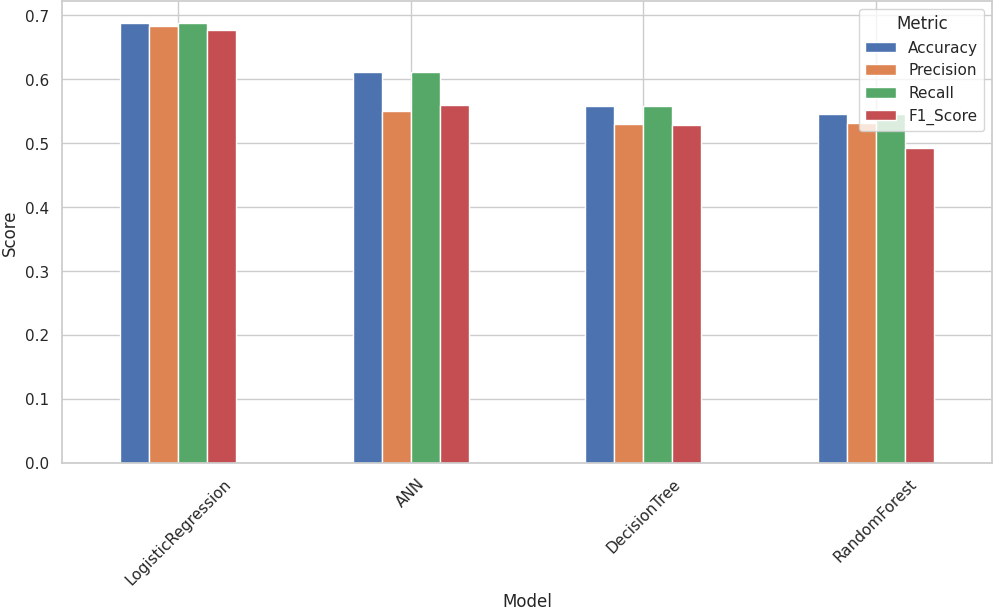
\includegraphics[width=0.8\textwidth]{fig/metics.png}
    \caption{Average Accuracy, Precision, Recall, F1-score per Model}
    \label{fig:metrics}
\end{figure}


Moreover, the pairplot presented in Figure~\ref{fig:pair_plot} offers a deeper view into the relationship between tested performance metrics. We can observe how the distributions of accuracy, precision, recall, and F1-score vary by model across all 324 datasets. A significant observation noted here is that we can see positive correlation between different metrics indicating that the performance of a model is consistent across all performance indicators. Logistic regression values cluster toward the higher end in each distribution, proving its robustness to different data configurations as shown also in Figure 1. When looking at distributions of performance of ANNs, we can observe that its performance is not consistent, the distribution shows that in many cases ANNs perform well and also in many of them them they achieve relatively low scores. On the other hand, Random forest demonstrates a fairly tight, centrally located cluster for each metric except precision, indicating consistent but not high performance.

\begin{figure}[h]
 \centering
    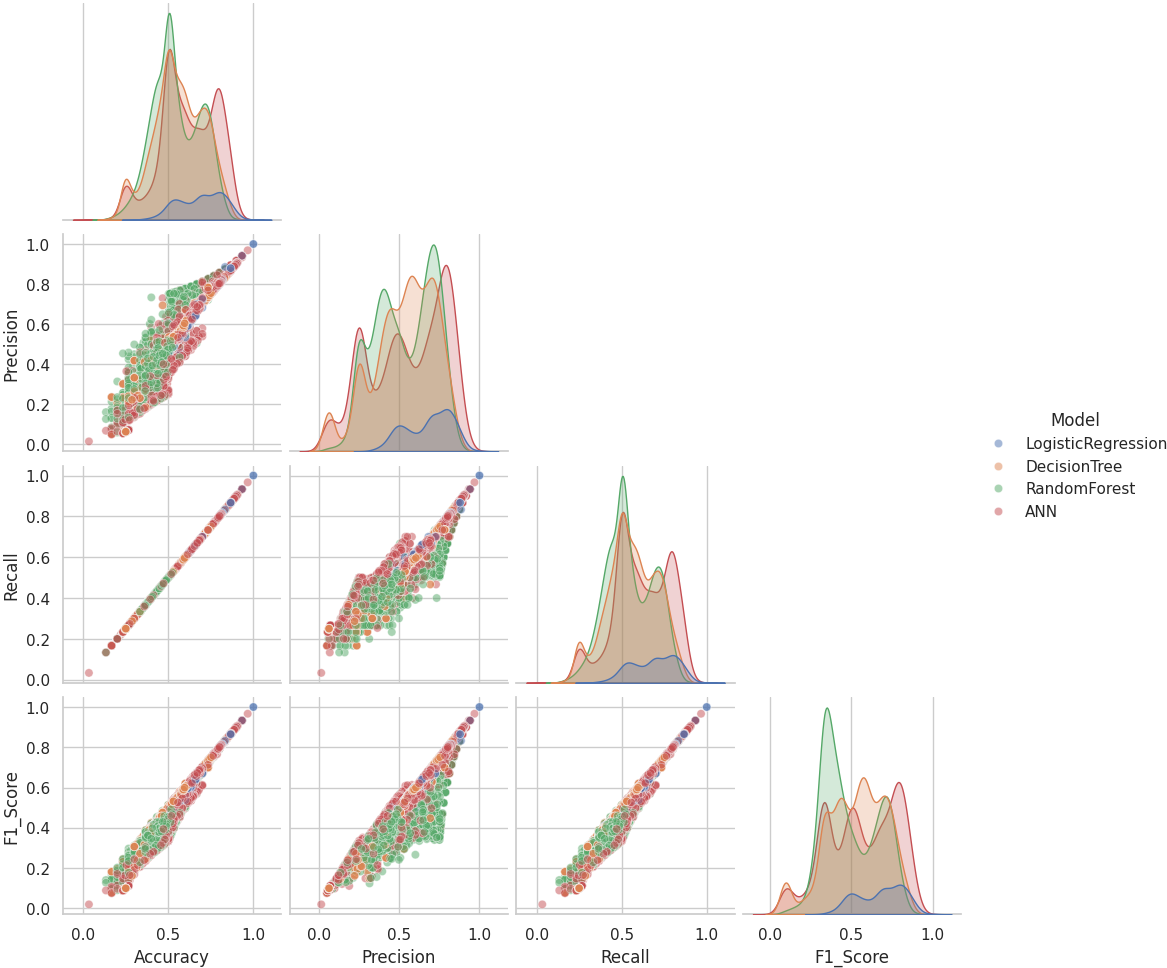
\includegraphics[width=0.8\textwidth]{fig/pair plots full.png}
    \caption{Pairplot of Performance Metrics}
    \label{fig:pair_plot}
\end{figure}

Finally, when comparing how performance metrics behave as the sample size increases, a few clear trends can be noticed based on Figure~\ref{fig:metrics_samplesize}. First, logistic regression consistently leads on all four metrics (accuracy, precision, recall, and F1‐score) regardless of the sample size. It also shows a steady improvement trend, suggesting good generalizability as more data becomes available. In contrast, the decision tree and random forest models both start off relatively close to chance levels for very small sample sizes, however, as more data becomes available for training their performance doesn't improve. The situation is very different with the ANNs where it has a comparatively poor start as well (compared to logistic regression), yet it makes a large jump around the sample size of 1000 (\(10^3\)), rapidly outperforming decision tree and random forest, however, still not overtaking logistic regression.  

\begin{figure}[h]
 \centering
    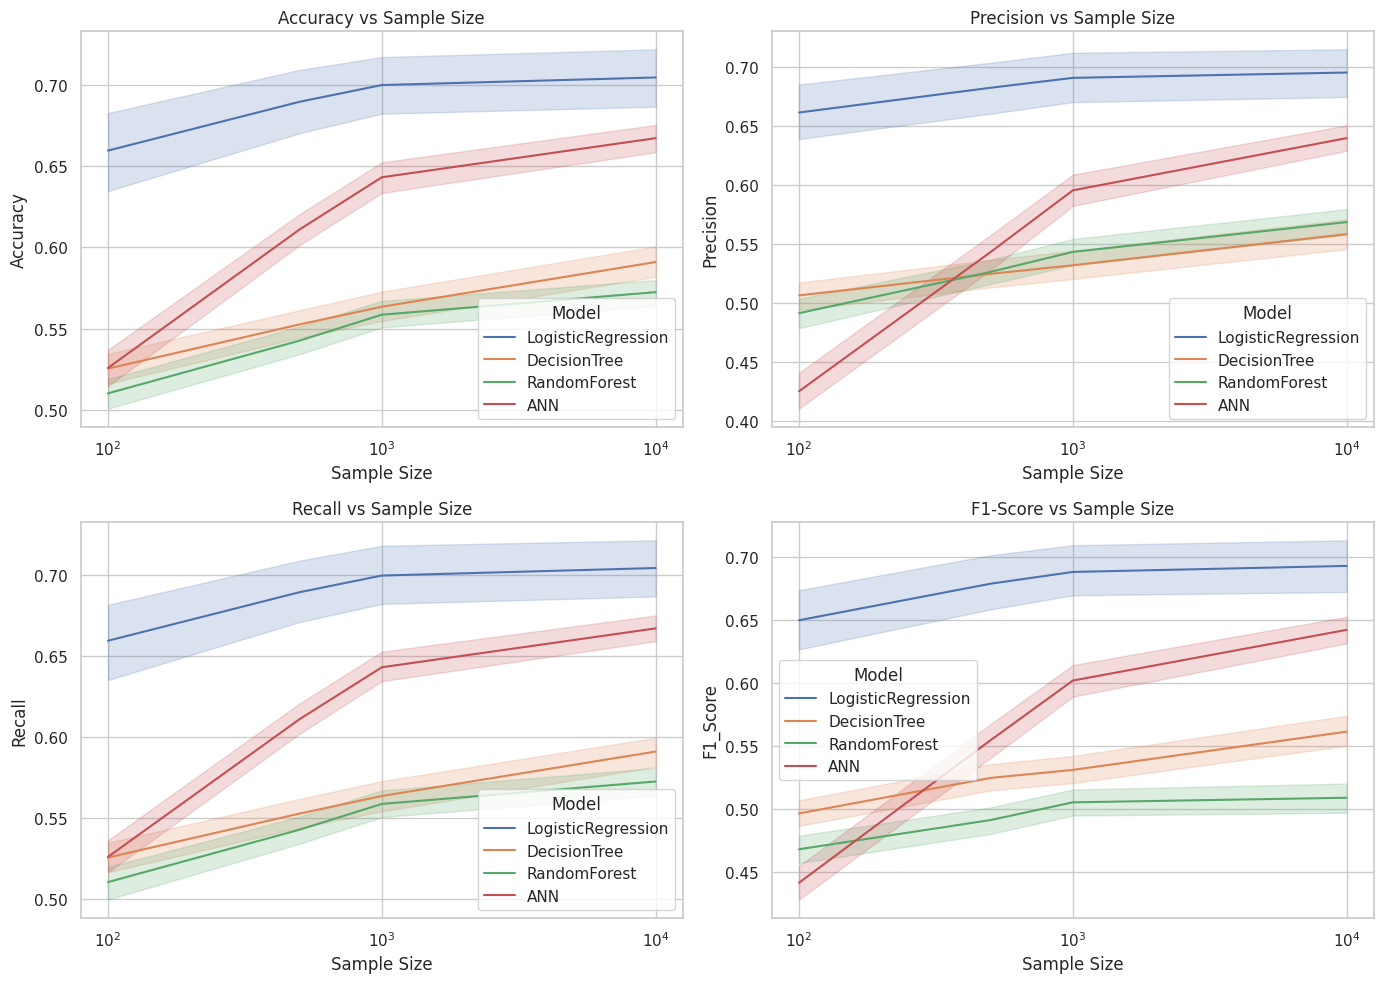
\includegraphics[width=0.8\textwidth]{fig/metrics vs sample size.png}
    \caption{Performance metrics vs sample size}
    \label{fig:metrics_samplesize}
\end{figure}

Overall, all models tend to improve as the sample size increases, but at different rates. This is consistent with Statistical Learning Theory, which holds that as the number of available data grows, the model’s performance should improve as proved by \textcite{Vapnik2015}. Logistic regression’s performance rises quickly and remains in the lead, indicating its robustness to both small and large datasets in our simulation. Meanwhile, the ANNs begin to truly shine once the sample size crosses a threshold of 1000 samples. The tree‐based models (decision tree and random forest) maintain relatively stable gains, but their improvement curves are not as pronounced, and they never quite match the top metrics that logistic regression achieves. Our results suggest that if one’s priority is consistently high performance across accuracy, precision, recall, and F1‐score, then logistic regression model is the most reliable choice based on the experiments performed in our simulation.

In the following section, in order to take a closer look into the detailed results we consider only the best performing hyperparameter configuration for each of the models tested. In this case we find ANNs to perform better than the other models. The performance of the models generally improve with increasing sample size (as in the case above), increasing number of categorical predictors, increasing number of predictor categories, and fewer outcome categories (see Figure~\ref{fig:15_mainEffects_V7} for the main effects in the case of seven predictors, including categorical ones).

    \begin{figure}[h]
        \centering
        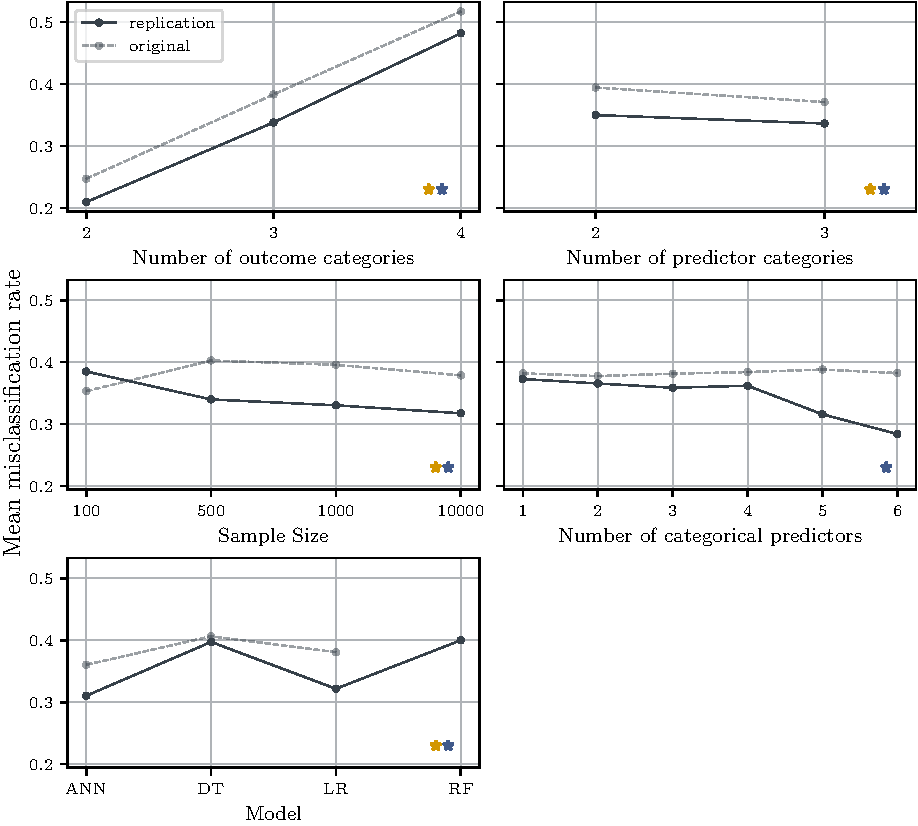
\includegraphics{fig/15_mainEffects_V7.pdf}
        \caption{Main Effects in the Case of Seven Predictors, Including Categorical Ones \\
        \textit{Note.} A yellow star indicates a significant effect in the original study, a blue star in the replication.}
        \label{fig:15_mainEffects_V7}
    \end{figure}


\subsection{Comparison with Main Results of \textcite{kim:10}}

    \paragraph{Main Result 1.}
    \textit{For continuous predictors, logistic regression was superior to ANN and decision tree when the outcome variable was binary, while the ANN was best when the number of outcome categories was three or more.}

    This result was not replicated (see Figure~\ref{fig:02_04_Interactions_cont} (a)). As in the original study, the misclassification rate increased with the number of outcome categories. However, in our replication the ANN always performed best, no matter the number of outcome categories. We did not find a significant interaction effect of model and number of outcome categories ($p$ = 0.464).

    \begin{figure}[h]
        \centering
        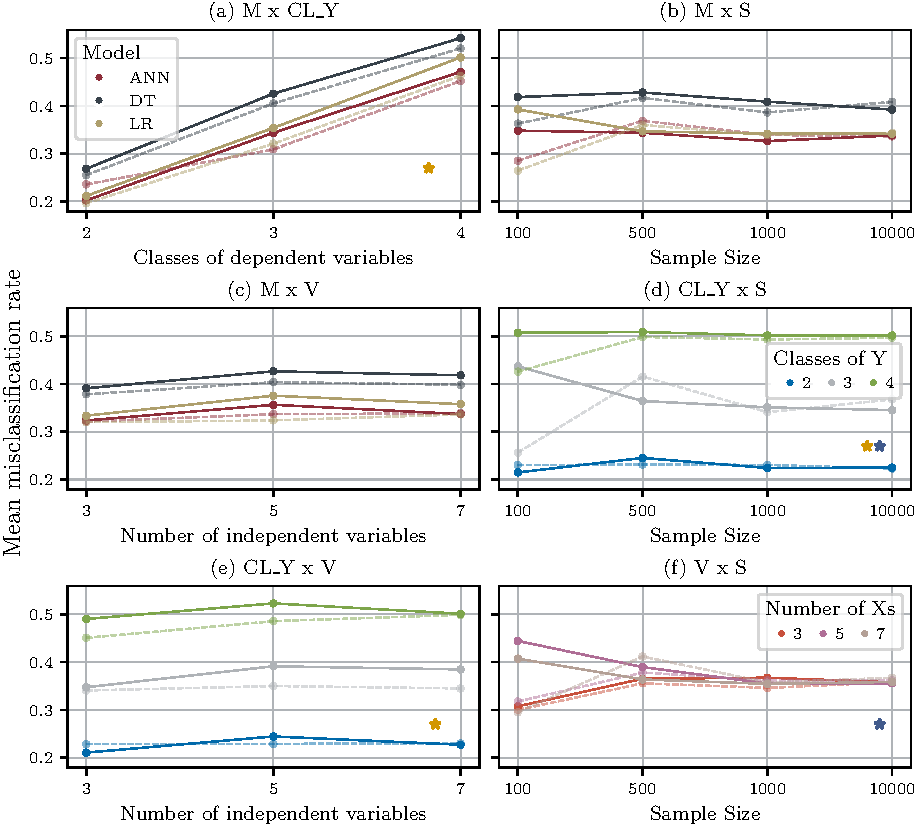
\includegraphics{fig/02_04_Interactions_cont.pdf}
        \caption{Interaction Plots for Datasets with Continuous Predictors \\
        \textit{Note.} M = model, CL\_Y = number of outcome categories, S = sample size, V = number of predictors}
        \label{fig:02_04_Interactions_cont}
    \end{figure}
    
    \paragraph{Main Result 2.}
    \textit{For continuous and categorical predictors, logistic regression performed better than ANN and decision tree in the case of a small number of predictors and a small sample size, while ANN was best in other cases.}

    This result was not replicated. We found no significant interaction between the model and the sample size in the case of three predictors (for details see Figure~\ref{fig:06_08_Interactions_V3} (c) in Appendix~\ref{app:figures}, $p$ = 0.403). Contrary to the original study, in the replication this interaction was significant in the case of five predictors, with logistic regression yielding slightly better results than ANN at sample size 100 (see Figure~\ref{fig:10_14_Interactions_V5} (c) Appendix~\ref{app:figures}). Except for this one case, ANN always performs better than the other two models.

    \paragraph{Main Result 3.}
    \textit{In the case of complex characteristics of the DGP, ANN was superior to the other methods.}

    This result was replicated in general. However, we found that ANN performed better even in the less complex cases and we found exceptions where logistic regression performed better than ANN in more complex cases (e.g., five predictors with four of them categorical, see Figure~\ref{fig:10_14_Interactions_V5} (d) Appendix~\ref{app:figures}). This yields caution in concluding that ANNs always perform better in more complex settings.
    
\section{Discussion}

We attempted to replicate \textcite{kim:10}, comparing three classification methods. When considering only the best hyperparameter configuration for each of the methods, we found that our ANN model had the best performance in most cases, while the decision tree had the worst performance. These results were consistent across various performance metrics. We replicated only one of the three main findings of the original study successfully, namely that ANNs perform best in more complex settings. 

Our inability to replicate the majority of the main findings of the original study highlights the significance of replications even for simulation studies in order to establish the reliability of their findings. The observed differences can be attributed to various potential sources. We identify four possible ones: First, the differences may be attributed to random variation. Both the original study and the replication, rely on a single iteration, making this a likely source to contribute to the differences. Second, the original study used the statistics software SAS for anlaysis, whereas we used Python in the replication. Model implementations may have changed, especially as these models have evolved over 15 years of research. Third, as previously mentioned, the ambiguity in some of the instructions concerning the DGP and the exact models left us guessing and is therefore another potential source of the differences. Finally, errors (e.g., in the code) in the original study or the replication could account for some of the differences. Ideally, we would now compare our code with the author's code and check where exactly the differences arise. Unfortunately, the code is not publicly available.

A replication is always a balancing act between adhering closely to the original study and adapting it to align with contemporary research practices. We decided to follow the original approach because we primary focused on demonstrating that simulation studies provide evidence rather than absolute facts. Closely following the original study and still being unable to replicate the majority of the main findings emphasizes this argument. This inevitably limits our contribution to contemporary research regarding which classification algorithm is most suitable for a given application.

This replication highlights two key lessons: skepticism and transparency. First, contrary to common assumptions, simulation studies cannot be taken as absolute truth. Even in this relatively straightforward neutral comparison study, we were able to replicate only one of the three main findings from the original study. Multiple replications and neutral comparison studies can help determine which method works best in different contexts, but a single simulation study rarely provides definitive evidence. Second, this study underscores the importance of making simulation code publicly available. As described, we had to make several assumptions about details of the DGP and the methods used, which complicated the replication process and made it difficult to pinpoint the exact sources of the differences in the results.

A more skeptical approach to simulation study results will lead to a more informed selection of appropriate methods, ultimately improving the quality and rigor of scientific research. At the same time, greater transparency in sharing code and methodological details will make it easier to assess and compare methods across studies, helping to build a more solid foundation for future research.

% \vskip 0.2in
% \newpage
\printbibliography


% Acknowledgements and Disclosure of Funding should go at the end, before appendices and references

% \newpage

% \acks{All acknowledgments go at the end of the paper before appendices and references.
% Moreover, you are required to declare funding (financial activities supporting the
% submitted work) and competing interests (related financial activities outside the submitted work).
% More information about this disclosure can be found on the JMLR website.}

% Manual newpage inserted to improve layout of sample file - not
% needed in general before appendices/bibliography.

\newpage

\appendix
\section{Detailed Tables of Misclassification Errors}
\label{app:misclass_errors}

{\small
\setlength{\tabcolsep}{3pt}
\renewcommand{\arraystretch}{1}
\begin{longtable}{ccccccccccccccc}
    \caption{\normalsize{Misclassification Errors for Continuous Predictors \\
         \textit{Note.} V = number of predictors, S = sample size, CL\_Y = number of outcome categories for ANN, decision tree (DT), logistic regression (LR), and random forest (RF)}} \\
    \hline
    V & S & \multicolumn{4}{c}{CL\_Y = 2} & \multicolumn{4}{c}{CL\_Y = 3} & \multicolumn{4}{c}{CL\_Y = 4} \\
    \cline{3-14}
    & & ANN & DT & LR & RF & ANN & DT & LR & RF & ANN & DT & LR & RF \\
    \hline
    3 & 100 & 0.100 & 0.233 & 0.133 & 0.167 & 0.260 & 0.387 & 0.227 & 0.167 & 0.347 & 0.447 & 0.467 & 0.600 \\
      & 500 & 0.180 & 0.313 & 0.180 & 0.247 & 0.367 & 0.433 & 0.333 & 0.247 & 0.400 & 0.467 & 0.447 & 0.607 \\
      & 1000 & 0.210 & 0.273 & 0.220 & 0.253 & 0.300 & 0.400 & 0.327 & 0.253 & 0.457 & 0.500 & 0.543 & 0.590 \\
      & 10000 & 0.221 & 0.239 & 0.222 & 0.249 & 0.329 & 0.393 & 0.332 & 0.249 & 0.480 & 0.528 & 0.498 & 0.564 \\
    \hline
    5 & 100 & 0.267 & 0.278 & 0.200 & 0.267 & 0.200 & 0.400 & 0.233 & 0.267 & 0.400 & 0.500 & 0.600 & 0.600 \\
      & 500 & 0.237 & 0.233 & 0.180 & 0.473 & 0.373 & 0.447 & 0.380 & 0.473 & 0.487 & 0.567 & 0.487 & 0.553 \\
      & 1000 & 0.247 & 0.263 & 0.227 & 0.460 & 0.310 & 0.399 & 0.343 & 0.460 & 0.513 & 0.536 & 0.487 & 0.520 \\
      & 10000 & 0.211 & 0.249 & 0.212 & 0.469 & 0.325 & 0.391 & 0.322 & 0.469 & 0.443 & 0.553 & 0.491 & 0.539 \\
    \hline
    7 & 100 & 0.267 & 0.256 & 0.233 & 0.487 & 0.167 & 0.267 & 0.200 & 0.487 & 0.433 & 0.500 & 0.500 & 0.633 \\
      & 500 & 0.270 & 0.230 & 0.167 & 0.447 & 0.393 & 0.493 & 0.393 & 0.447 & 0.527 & 0.557 & 0.477 & 0.600 \\
      & 1000 & 0.207 & 0.320 & 0.200 & 0.472 & 0.310 & 0.354 & 0.330 & 0.472 & 0.477 & 0.510 & 0.477 & 0.543 \\
      & 10000 & 0.206 & 0.254 & 0.206 & 0.472 & 0.337 & 0.449 & 0.341 & 0.472 & 0.463 & 0.561 & 0.469 & 0.558 \\
    \hline
    \label{tab:misclassification_errors}
\end{longtable}
}

{\small
\setlength{\tabcolsep}{3pt}
\renewcommand{\arraystretch}{1}
\begin{longtable}{ccccccccccccccc}
    \caption{\normalsize{Misclassification Errors for DGPs with Three Predictors (Including Categorical) \\
         \textit{Note.} CA = number of categorical predictors, CL\_X = number of categories for categorical predictors}} \\
    \hline
    CA & CL\_X & S & \multicolumn{4}{c}{CL\_Y = 2} & \multicolumn{4}{c}{CL\_Y = 3} & \multicolumn{4}{c}{CL\_Y = 4} \\
    \cline{4-15}
    & & & ANN & DT & LR & RF & ANN & DT & LR & RF & ANN & DT & LR & RF \\
    \hline
    1 & 2 & 100 & 0.200 & 0.167 & 0.300 & 0.267 & 0.333 & 0.367 & 0.367 & 0.333 & 0.400 & 0.433 & 0.400 & 0.467 \\
      &   & 500 & 0.240 & 0.293 & 0.240 & 0.247 & 0.313 & 0.367 & 0.287 & 0.420 & 0.433 & 0.500 & 0.440 & 0.533 \\
      &   & 1000 & 0.147 & 0.180 & 0.160 & 0.167 & 0.257 & 0.337 & 0.243 & 0.473 & 0.413 & 0.457 & 0.457 & 0.547 \\
      &   & 10000 & 0.181 & 0.199 & 0.184 & 0.209 & 0.307 & 0.330 & 0.308 & 0.490 & 0.426 & 0.436 & 0.458 & 0.529 \\
    \hline
    1 & 3 & 100 & 0.133 & 0.133 & 0.167 & 0.233 & 0.400 & 0.433 & 0.300 & 0.267 & 0.367 & 0.400 & 0.500 & 0.433 \\
      &   & 500 & 0.127 & 0.127 & 0.147 & 0.193 & 0.207 & 0.333 & 0.227 & 0.287 & 0.413 & 0.447 & 0.413 & 0.480 \\
      &   & 1000 & 0.167 & 0.197 & 0.160 & 0.187 & 0.240 & 0.290 & 0.230 & 0.317 & 0.340 & 0.393 & 0.403 & 0.430 \\
      &   & 10000 & 0.150 & 0.168 & 0.153 & 0.202 & 0.237 & 0.266 & 0.241 & 0.336 & 0.380 & 0.410 & 0.407 & 0.459 \\
    \hline
    2 & 2 & 100 & 0.133 & 0.300 & 0.233 & 0.067 & 0.233 & 0.300 & 0.233 & 0.400 & 0.367 & 0.267 & 0.333 & 0.400 \\
      &   & 500 & 0.160 & 0.187 & 0.167 & 0.187 & 0.253 & 0.273 & 0.253 & 0.453 & 0.407 & 0.433 & 0.420 & 0.507 \\
      &   & 1000 & 0.167 & 0.220 & 0.173 & 0.177 & 0.247 & 0.290 & 0.263 & 0.480 & 0.437 & 0.487 & 0.473 & 0.520 \\
      &   & 10000 & 0.146 & 0.150 & 0.148 & 0.149 & 0.264 & 0.266 & 0.264 & 0.500 & 0.409 & 0.412 & 0.423 & 0.521 \\
    \hline
    2 & 3 & 100 & 0.133 & 0.267 & 0.133 & 0.233 & 0.233 & 0.300 & 0.200 & 0.300 & 0.267 & 0.400 & 0.300 & 0.467 \\
      &   & 500 & 0.133 & 0.200 & 0.133 & 0.207 & 0.187 & 0.200 & 0.207 & 0.380 & 0.347 & 0.447 & 0.393 & 0.440 \\
      &   & 1000 & 0.107 & 0.173 & 0.113 & 0.183 & 0.183 & 0.257 & 0.183 & 0.353 & 0.303 & 0.380 & 0.350 & 0.420 \\
      &   & 10000 & 0.130 & 0.131 & 0.131 & 0.169 & 0.200 & 0.208 & 0.200 & 0.389 & 0.344 & 0.354 & 0.368 & 0.500 \\
    \hline
    \label{tab:misclassification_errors}
\end{longtable}
}


{\small
\setlength{\tabcolsep}{3pt}
\renewcommand{\arraystretch}{1}
\begin{longtable}{ccccccccccccccc}
    \caption{\normalsize{Misclassification Errors for DGPs with Five Predictors (Including Categorical)}} \\
    \hline
    CA & CL\_X & S & \multicolumn{4}{c}{CL\_Y = 2} & \multicolumn{4}{c}{CL\_Y = 3} & \multicolumn{4}{c}{CL\_Y = 4} \\
    \cline{4-15}
    & & & ANN & DT & LR & RF & ANN & DT & LR & RF & ANN & DT & LR & RF \\
    \hline
    1 & 2 & 100 & 0.200 & 0.267 & 0.200 & 0.167 & 0.367 & 0.433 & 0.500 & 0.467 & 0.533 & 0.567 & 0.533 & 0.467 \\
      &   & 500 & 0.267 & 0.293 & 0.253 & 0.247 & 0.320 & 0.400 & 0.353 & 0.427 & 0.487 & 0.520 & 0.520 & 0.533 \\
      &   & 1000 & 0.187 & 0.267 & 0.183 & 0.237 & 0.323 & 0.417 & 0.320 & 0.440 & 0.453 & 0.543 & 0.487 & 0.523 \\
      &   & 10000 & 0.198 & 0.239 & 0.201 & 0.253 & 0.313 & 0.375 & 0.316 & 0.392 & 0.436 & 0.531 & 0.454 & 0.532 \\
    \hline
    1 & 3 & 100 & 0.233 & 0.267 & 0.300 & 0.300 & 0.467 & 0.533 & 0.533 & 0.433 & 0.367 & 0.467 & 0.367 & 0.467 \\
      &   & 500 & 0.187 & 0.307 & 0.200 & 0.260 & 0.347 & 0.413 & 0.373 & 0.413 & 0.447 & 0.607 & 0.473 & 0.547 \\
      &   & 1000 & 0.157 & 0.247 & 0.163 & 0.200 & 0.313 & 0.427 & 0.310 & 0.410 & 0.410 & 0.557 & 0.437 & 0.540 \\
      &   & 10000 & 0.183 & 0.224 & 0.187 & 0.240 & 0.296 & 0.366 & 0.293 & 0.396 & 0.440 & 0.517 & 0.452 & 0.526 \\
    \hline
    2 & 2 & 100 & 0.133 & 0.133 & 0.167 & 0.100 & 0.367 & 0.400 & 0.433 & 0.367 & 0.400 & 0.533 & 0.400 & 0.567 \\
      &   & 500 & 0.187 & 0.233 & 0.207 & 0.267 & 0.260 & 0.427 & 0.287 & 0.400 & 0.460 & 0.520 & 0.473 & 0.527 \\
      &   & 1000 & 0.180 & 0.280 & 0.180 & 0.240 & 0.280 & 0.410 & 0.283 & 0.423 & 0.457 & 0.567 & 0.483 & 0.523 \\
      &   & 10000 & 0.186 & 0.231 & 0.183 & 0.222 & 0.310 & 0.368 & 0.308 & 0.369 & 0.446 & 0.516 & 0.478 & 0.525 \\
    \hline
    2 & 3 & 100 & 0.067 & 0.233 & 0.133 & 0.167 & 0.267 & 0.333 & 0.167 & 0.300 & 0.467 & 0.467 & 0.400 & 0.500 \\
      &   & 500 & 0.220 & 0.313 & 0.227 & 0.253 & 0.287 & 0.407 & 0.273 & 0.373 & 0.380 & 0.540 & 0.393 & 0.480 \\
      &   & 1000 & 0.210 & 0.293 & 0.190 & 0.277 & 0.273 & 0.430 & 0.280 & 0.427 & 0.403 & 0.557 & 0.447 & 0.523 \\
      &   & 10000 & 0.182 & 0.227 & 0.180 & 0.224 & 0.266 & 0.345 & 0.263 & 0.387 & 0.422 & 0.509 & 0.442 & 0.516 \\
    \hline
    3 & 2 & 100 & 0.033 & 0.233 & 0.000 & 0.167 & 0.233 & 0.333 & 0.233 & 0.400 & 0.467 & 0.533 & 0.467 & 0.433 \\
      &   & 500 & 0.147 & 0.227 & 0.167 & 0.213 & 0.233 & 0.433 & 0.260 & 0.353 & 0.427 & 0.507 & 0.447 & 0.500 \\
      &   & 1000 & 0.183 & 0.253 & 0.183 & 0.253 & 0.307 & 0.337 & 0.287 & 0.333 & 0.383 & 0.477 & 0.437 & 0.487 \\
      &   & 10000 & 0.174 & 0.203 & 0.174 & 0.222 & 0.253 & 0.293 & 0.265 & 0.304 & 0.408 & 0.453 & 0.439 & 0.514 \\
    \hline
    3 & 3 & 100 & 0.167 & 0.367 & 0.100 & 0.267 & 0.400 & 0.467 & 0.367 & 0.400 & 0.300 & 0.400 & 0.433 & 0.433 \\
      &   & 500 & 0.120 & 0.220 & 0.127 & 0.193 & 0.260 & 0.340 & 0.247 & 0.367 & 0.387 & 0.487 & 0.420 & 0.513 \\
      &   & 1000 & 0.140 & 0.210 & 0.150 & 0.210 & 0.233 & 0.333 & 0.243 & 0.387 & 0.373 & 0.457 & 0.373 & 0.487 \\
      &   & 10000 & 0.136 & 0.169 & 0.135 & 0.176 & 0.233 & 0.275 & 0.226 & 0.325 & 0.356 & 0.433 & 0.371 & 0.492 \\
    \hline
    4 & 2 & 100 & 0.067 & 0.200 & 0.067 & 0.133 & 0.233 & 0.367 & 0.233 & 0.367 & 0.400 & 0.500 & 0.333 & 0.400 \\
      &   & 500 & 0.127 & 0.200 & 0.133 & 0.167 & 0.287 & 0.373 & 0.313 & 0.333 & 0.360 & 0.487 & 0.427 & 0.507 \\
      &   & 1000 & 0.117 & 0.177 & 0.127 & 0.180 & 0.237 & 0.303 & 0.233 & 0.347 & 0.393 & 0.443 & 0.407 & 0.473 \\
      &   & 10000 & 0.144 & 0.154 & 0.149 & 0.151 & 0.252 & 0.265 & 0.250 & 0.317 & 0.365 & 0.390 & 0.394 & 0.473 \\
    \hline
    4 & 3 & 100 & 0.200 & 0.367 & 0.133 & 0.233 & 0.467 & 0.400 & 0.267 & 0.400 & 0.433 & 0.433 & 0.300 & 0.333 \\
      &   & 500 & 0.127 & 0.193 & 0.140 & 0.160 & 0.220 & 0.300 & 0.207 & 0.373 & 0.300 & 0.440 & 0.353 & 0.467 \\
      &   & 1000 & 0.107 & 0.187 & 0.110 & 0.180 & 0.193 & 0.247 & 0.183 & 0.303 & 0.343 & 0.430 & 0.400 & 0.470 \\
      &   & 10000 & 0.130 & 0.157 & 0.128 & 0.194 & 0.189 & 0.242 & 0.187 & 0.287 & 0.311 & 0.377 & 0.344 & 0.487 \\
    \hline
    \label{tab:misclassification_errors}
\end{longtable}
}

{\small
\setlength{\tabcolsep}{3pt}
\renewcommand{\arraystretch}{1}
\begin{longtable}{ccccccccccccccc}
    \caption{\normalsize{Misclassification Errors for DGPs with Seven Predictors (Including Categorical)}} \\
    \hline
    CA & CL\_X & S & \multicolumn{4}{c}{CL\_Y = 2} & \multicolumn{4}{c}{CL\_Y = 3} & \multicolumn{4}{c}{CL\_Y = 4} \\
    \cline{4-15}
    & & & ANN & DT & LR & RF & ANN & DT & LR & RF & ANN & DT & LR & RF \\
    \hline
    1 & 2 & 100 & 0.200 & 0.333 & 0.233 & 0.300 & 0.433 & 0.400 & 0.333 & 0.367 & 0.567 & 0.667 & 0.633 & 0.600 \\
      &   & 500 & 0.240 & 0.320 & 0.260 & 0.293 & 0.287 & 0.413 & 0.333 & 0.460 & 0.480 & 0.540 & 0.507 & 0.587 \\
      &   & 1000 & 0.210 & 0.270 & 0.213 & 0.267 & 0.317 & 0.450 & 0.300 & 0.463 & 0.487 & 0.583 & 0.493 & 0.570 \\
      &   & 10000 & 0.205 & 0.254 & 0.204 & 0.252 & 0.318 & 0.405 & 0.315 & 0.433 & 0.460 & 0.546 & 0.475 & 0.543 \\
    \hline
    1 & 3 & 100 & 0.267 & 0.400 & 0.300 & 0.233 & 0.367 & 0.400 & 0.367 & 0.367 & 0.533 & 0.567 & 0.567 & 0.600 \\
      &   & 500 & 0.187 & 0.267 & 0.193 & 0.273 & 0.327 & 0.380 & 0.293 & 0.407 & 0.420 & 0.467 & 0.427 & 0.533 \\
      &   & 1000 & 0.190 & 0.303 & 0.193 & 0.277 & 0.300 & 0.437 & 0.300 & 0.467 & 0.450 & 0.577 & 0.490 & 0.560 \\
      &   & 10000 & 0.199 & 0.261 & 0.200 & 0.239 & 0.322 & 0.394 & 0.318 & 0.420 & 0.460 & 0.558 & 0.472 & 0.549 \\
    \hline
    2 & 2 & 100 & 0.167 & 0.233 & 0.167 & 0.367 & 0.400 & 0.533 & 0.333 & 0.367 & 0.467 & 0.467 & 0.467 & 0.633 \\
      &   & 500 & 0.220 & 0.287 & 0.227 & 0.220 & 0.347 & 0.407 & 0.367 & 0.420 & 0.493 & 0.580 & 0.500 & 0.587 \\
      &   & 1000 & 0.167 & 0.263 & 0.173 & 0.223 & 0.273 & 0.397 & 0.300 & 0.407 & 0.430 & 0.547 & 0.457 & 0.563 \\
      &   & 10000 & 0.205 & 0.255 & 0.208 & 0.258 & 0.315 & 0.400 & 0.311 & 0.434 & 0.451 & 0.543 & 0.462 & 0.545 \\
    \hline
    2 & 3 & 100 & 0.200 & 0.300 & 0.267 & 0.167 & 0.400 & 0.467 & 0.500 & 0.467 & 0.533 & 0.533 & 0.533 & 0.533 \\
      &   & 500 & 0.207 & 0.307 & 0.173 & 0.287 & 0.313 & 0.420 & 0.313 & 0.440 & 0.493 & 0.567 & 0.487 & 0.573 \\
      &   & 1000 & 0.200 & 0.293 & 0.203 & 0.270 & 0.323 & 0.460 & 0.313 & 0.470 & 0.470 & 0.587 & 0.483 & 0.570 \\
      &   & 10000 & 0.197 & 0.252 & 0.203 & 0.240 & 0.318 & 0.402 & 0.310 & 0.451 & 0.451 & 0.542 & 0.477 & 0.539 \\
    \hline
    3 & 2 & 100 & 0.067 & 0.233 & 0.067 & 0.200 & 0.300 & 0.500 & 0.267 & 0.300 & 0.467 & 0.467 & 0.633 & 0.600 \\
      &   & 500 & 0.173 & 0.293 & 0.187 & 0.287 & 0.347 & 0.460 & 0.373 & 0.460 & 0.473 & 0.513 & 0.467 & 0.573 \\
      &   & 1000 & 0.183 & 0.257 & 0.193 & 0.240 & 0.317 & 0.433 & 0.320 & 0.453 & 0.447 & 0.560 & 0.490 & 0.567 \\
      &   & 10000 & 0.189 & 0.242 & 0.188 & 0.243 & 0.309 & 0.387 & 0.311 & 0.416 & 0.466 & 0.541 & 0.478 & 0.557 \\
    \hline
    3 & 3 & 100 & 0.267 & 0.300 & 0.233 & 0.200 & 0.333 & 0.500 & 0.500 & 0.433 & 0.533 & 0.633 & 0.600 & 0.500 \\
      &   & 500 & 0.213 & 0.280 & 0.240 & 0.267 & 0.300 & 0.420 & 0.300 & 0.440 & 0.407 & 0.600 & 0.433 & 0.567 \\
      &   & 1000 & 0.203 & 0.293 & 0.213 & 0.270 & 0.280 & 0.403 & 0.303 & 0.443 & 0.417 & 0.563 & 0.460 & 0.553 \\
      &   & 10000 & 0.191 & 0.242 & 0.195 & 0.238 & 0.304 & 0.375 & 0.309 & 0.458 & 0.419 & 0.526 & 0.433 & 0.541 \\
    \hline
    4 & 2 & 100 & 0.133 & 0.267 & 0.133 & 0.200 & 0.333 & 0.467 & 0.333 & 0.367 & 0.467 & 0.533 & 0.533 & 0.567 \\
      &   & 500 & 0.187 & 0.267 & 0.193 & 0.273 & 0.327 & 0.380 & 0.293 & 0.407 & 0.420 & 0.467 & 0.427 & 0.533 \\
      &   & 1000 & 0.190 & 0.303 & 0.193 & 0.277 & 0.300 & 0.437 & 0.300 & 0.467 & 0.450 & 0.577 & 0.490 & 0.560 \\
      &   & 10000 & 0.199 & 0.261 & 0.200 & 0.239 & 0.322 & 0.394 & 0.318 & 0.420 & 0.460 & 0.558 & 0.472 & 0.549 \\
    \hline
    4 & 3 & 100 & 0.200 & 0.300 & 0.267 & 0.167 & 0.400 & 0.467 & 0.500 & 0.467 & 0.533 & 0.533 & 0.533 & 0.533 \\
      &   & 500 & 0.207 & 0.307 & 0.173 & 0.287 & 0.313 & 0.420 & 0.313 & 0.440 & 0.493 & 0.567 & 0.487 & 0.573 \\
      &   & 1000 & 0.200 & 0.293 & 0.203 & 0.270 & 0.323 & 0.460 & 0.313 & 0.470 & 0.470 & 0.587 & 0.483 & 0.570 \\
      &   & 10000 & 0.197 & 0.252 & 0.203 & 0.240 & 0.318 & 0.402 & 0.310 & 0.451 & 0.451 & 0.542 & 0.477 & 0.539 \\
    \hline
    5 & 2 & 100 & 0.133 & 0.267 & 0.133 & 0.200 & 0.333 & 0.467 & 0.333 & 0.367 & 0.467 & 0.533 & 0.533 & 0.567 \\
      &   & 500 & 0.187 & 0.267 & 0.193 & 0.273 & 0.327 & 0.380 & 0.293 & 0.407 & 0.420 & 0.467 & 0.427 & 0.533 \\
      &   & 1000 & 0.190 & 0.303 & 0.193 & 0.277 & 0.300 & 0.437 & 0.300 & 0.467 & 0.450 & 0.577 & 0.490 & 0.560 \\
      &   & 10000 & 0.199 & 0.261 & 0.200 & 0.239 & 0.322 & 0.394 & 0.318 & 0.420 & 0.460 & 0.558 & 0.472 & 0.549 \\
    \hline
    5 & 3 & 100 & 0.200 & 0.300 & 0.267 & 0.167 & 0.400 & 0.467 & 0.500 & 0.467 & 0.533 & 0.533 & 0.533 & 0.533 \\
      &   & 500 & 0.207 & 0.307 & 0.173 & 0.287 & 0.313 & 0.420 & 0.313 & 0.440 & 0.493 & 0.567 & 0.487 & 0.573 \\
      &   & 1000 & 0.200 & 0.293 & 0.203 & 0.270 & 0.323 & 0.460 & 0.313 & 0.470 & 0.470 & 0.587 & 0.483 & 0.570 \\
      &   & 10000 & 0.197 & 0.252 & 0.203 & 0.240 & 0.318 & 0.402 & 0.310 & 0.451 & 0.451 & 0.542 & 0.477 & 0.539 \\
    \hline
    6 & 2 & 100 & 0.133 & 0.267 & 0.133 & 0.200 & 0.333 & 0.467 & 0.333 & 0.367 & 0.467 & 0.533 & 0.533 & 0.567 \\
      &   & 500 & 0.187 & 0.267 & 0.193 & 0.273 & 0.327 & 0.380 & 0.293 & 0.407 & 0.420 & 0.467 & 0.427 & 0.533 \\
      &   & 1000 & 0.190 & 0.303 & 0.193 & 0.277 & 0.300 & 0.437 & 0.300 & 0.467 & 0.450 & 0.577 & 0.490 & 0.560 \\
      &   & 10000 & 0.199 & 0.261 & 0.200 & 0.239 & 0.322 & 0.394 & 0.318 & 0.420 & 0.460 & 0.558 & 0.472 & 0.549 \\
    \hline
    6 & 3 & 100 & 0.200 & 0.300 & 0.267 & 0.167 & 0.400 & 0.467 & 0.500 & 0.467 & 0.533 & 0.533 & 0.533 & 0.533 \\
      &   & 500 & 0.207 & 0.307 & 0.173 & 0.287 & 0.313 & 0.420 & 0.313 & 0.440 & 0.493 & 0.567 & 0.487 & 0.573 \\
      &   & 1000 & 0.200 & 0.293 & 0.203 & 0.270 & 0.323 & 0.460 & 0.313 & 0.470 & 0.470 & 0.587 & 0.483 & 0.570 \\
      &   & 10000 & 0.197 & 0.252 & 0.203 & 0.240 & 0.318 & 0.402 & 0.310 & 0.451 & 0.451 & 0.542 & 0.477 & 0.539 \\
    \hline
    \label{tab:misclassification_errors}
\end{longtable}
}

\newpage
\section{ANOVA Tables}
\label{app:anova_tables}

\begin{table}[h]
    \centering
    \caption{ANOVA Table for DGPs with Continuous Predictors Only}
    \label{tab:anova_cont}
    \vspace{0.2cm}
    \begin{tabular}{lrrrr}
        \toprule
        Source & SS & df & F & $p$ \\
        \midrule
        CL\_Y           & 1.390  & 2  & 707.300  & $<$ .001 \\
        V              & 0.025  & 2  & 12.536   & $<$ .001 \\
        S              & 0.015  & 3  & 5.079    & .003  \\
        Model          & 0.105  & 2  & 53.535   & $<$ .001 \\
        CL\_Y $\times$ V      & 0.002  & 4  & 0.595    & .668  \\
        CL\_Y $\times$ S      & 0.039  & 6  & 6.534    & $<$ .001 \\
        CL\_Y $\times$ Model  & 0.004  & 4  & 0.909    & .464  \\
        V $\times$ S         & 0.071  & 6  & 11.985   & $<$ .001 \\
        V $\times$ Model     & 0.001  & 4  & 0.223    & .925  \\
        S $\times$ Model     & 0.010  & 6  & 1.738    & .125  \\
        Residual       & 0.067  & 68 & ---       & ---    \\
        \bottomrule
    \end{tabular}
\end{table}

\begin{table}[h]
    \centering
    \caption{ANOVA Table for DGP with Three Predictors (Including Categorical)}
    \label{tab:anova_v3}
    \vspace{0.2cm}
    \begin{tabular}{lrrrr}
        \toprule
        Source & SS & df & F & $p$ \\
        \midrule
        CL\_Y           & 1.261  & 2   & 490.181  & $<$ .001 \\
        CL\_X           & 0.065  & 1   & 50.185   & $<$ .001 \\
        S              & 0.009  & 3   & 2.312    & .081  \\
        CA             & 0.057  & 1   & 44.641   & $<$ .001 \\
        Model          & 0.041  & 2   & 16.069   & $<$ .001 \\
        CL\_Y $\times$ CL\_X  & 0.000  & 2   & 0.024    & .976  \\
        CL\_Y $\times$ S      & 0.044  & 6   & 5.751    & $<$ .001 \\
        CL\_Y $\times$ CA     & 0.014  & 2   & 5.584    & .005  \\
        CL\_Y $\times$ Model  & 0.009  & 4   & 1.737    & .148  \\
        CL\_X $\times$ S      & 0.008  & 3   & 2.134    & .101  \\
        CL\_X $\times$ CA     & 0.000  & 1   & 0.107    & .744  \\
        CL\_X $\times$ Model  & 0.003  & 2   & 0.959    & .387  \\
        S $\times$ CA         & 0.011  & 3   & 2.951    & .036  \\
        S $\times$ Model      & 0.008  & 6   & 1.041    & .403  \\
        CA $\times$ Model     & 0.001  & 2   & 0.492    & .613  \\
        Residual       & 0.133  & 103  & ---       & ---    \\
        \bottomrule
    \end{tabular}
\end{table}

\begin{table}[h]
    \centering
    \caption{ANOVA Table for DGP with Five Predictors (Including Categorical)}
    \label{tab:anova_v5}
    \vspace{0.2cm}
    \begin{tabular}{lrrrr}
        \toprule
        Source & SS & df & F & $p$ \\
        \midrule
        CL\_Y           & 3.131  & 2   & 894.594  & $<$ .001 \\
        CL\_X           & 0.012  & 1   & 6.854    & .009  \\
        S              & 0.043  & 3   & 8.270    & $<$ .001 \\
        CA             & 0.347  & 3   & 66.139   & $<$ .001 \\
        Model          & 0.383  & 2   & 109.363  & $<$ .001 \\
        CL\_Y $\times$ CL\_X  & 0.030  & 2   & 8.590    & $<$ .001 \\
        CL\_Y $\times$ S      & 0.070  & 6   & 6.628    & $<$ .001 \\
        CL\_Y $\times$ CA     & 0.016  & 6   & 1.562    & .159  \\
        CL\_Y $\times$ Model  & 0.003  & 4   & 0.417    & .796  \\
        CL\_X $\times$ S      & 0.020  & 3   & 3.801    & .011  \\
        CL\_X $\times$ CA     & 0.001  & 3   & 0.160    & .923  \\
        CL\_X $\times$ Model  & 0.006  & 2   & 1.825    & .164  \\
        S $\times$ CA         & 0.056  & 9   & 3.558    & $<$ .001 \\
        S $\times$ Model      & 0.023  & 6   & 2.230    & .041  \\
        CA $\times$ Model     & 0.009  & 6   & 0.822    & .554  \\
        Residual       & 0.401  & 229  & ---       & ---    \\
        \bottomrule
    \end{tabular}
\end{table}

\begin{table}[h]
    \centering
    \caption{ANOVA Table for DGP with Seven Predictors (Including Categorical)}
    \label{tab:anova_v7}
    \vspace{0.2cm}
    \begin{tabular}{lrrrr}
        \toprule
        Source & SS & df & F & p \\
        \midrule
        CL\_Y           & 5.349  & 2   & 2225.790  & $<$ .001 \\
        CL\_X           & 0.020  & 1   & 16.879    & $<$ .001 \\
        S              & 0.279  & 3   & 77.358    & $<$ .001 \\
        CA             & 0.448  & 5   & 74.575    & $<$ .001 \\
        Model          & 0.643  & 2   & 267.419   & $<$ .001 \\
        CL\_Y $\times$ CL\_X  & 0.007  & 2   & 2.953    & .054  \\
        CL\_Y $\times$ S      & 0.027  & 6   & 3.733    & .001  \\
        CL\_Y $\times$ CA     & 0.032  & 10  & 2.643    & .004  \\
        CL\_Y $\times$ Model  & 0.019  & 4   & 3.863    & .004  \\
        CL\_X $\times$ S      & 0.044  & 3   & 12.111   & $<$ .001 \\
        CL\_X $\times$ CA     & 0.065  & 5   & 10.806   & $<$ .001 \\
        CL\_X $\times$ Model  & 0.003  & 2   & 1.419    & .243  \\
        S $\times$ CA         & 0.038  & 15  & 2.118    & .009  \\
        S $\times$ Model      & 0.014  & 6   & 1.868    & .086  \\
        CA $\times$ Model     & 0.006  & 10  & 0.487    & .898  \\
        Residual       & 0.427  & 355  & ---       & ---    \\
        \bottomrule
    \end{tabular}
\end{table}


\clearpage
\section{Additional Figures}
\label{app:figures}

\begin{figure}[h]
    \centering
    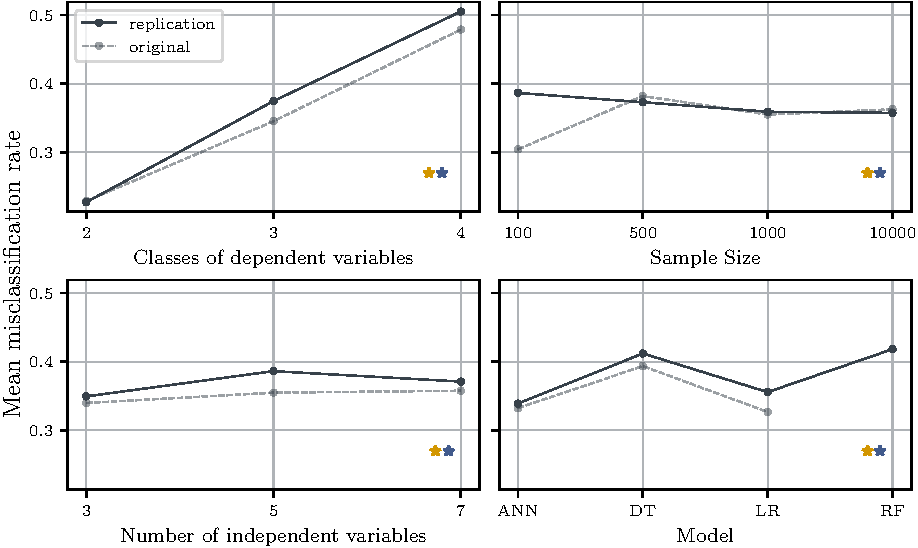
\includegraphics{fig/01_mainEffects_cont.pdf}
    \caption{Main Effects for Datasets with Continuous Predictors}
    \label{fig:01_mainEffects_cont}
\end{figure}

\begin{figure}[h]
    \centering
    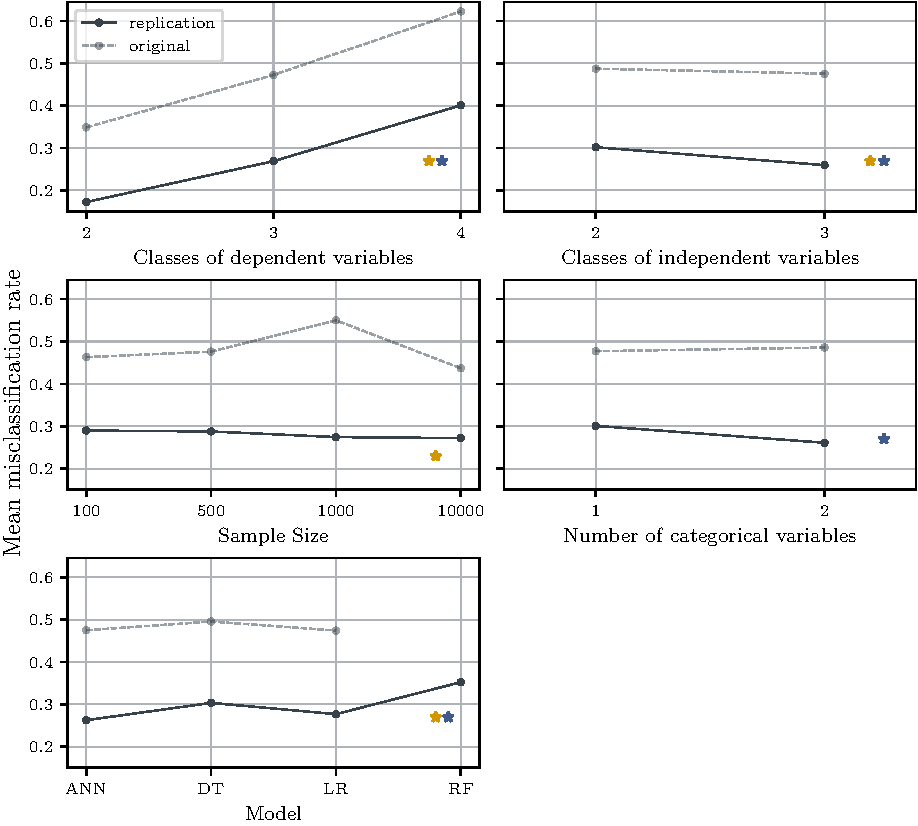
\includegraphics{fig/05_mainEffects_V3.pdf}
    \caption{Main Effects for Datasets with Three Predictors (Including Categorical Ones)}
    \label{fig:05_mainEffects_V3}
\end{figure}

\begin{figure}[h]
    \centering
    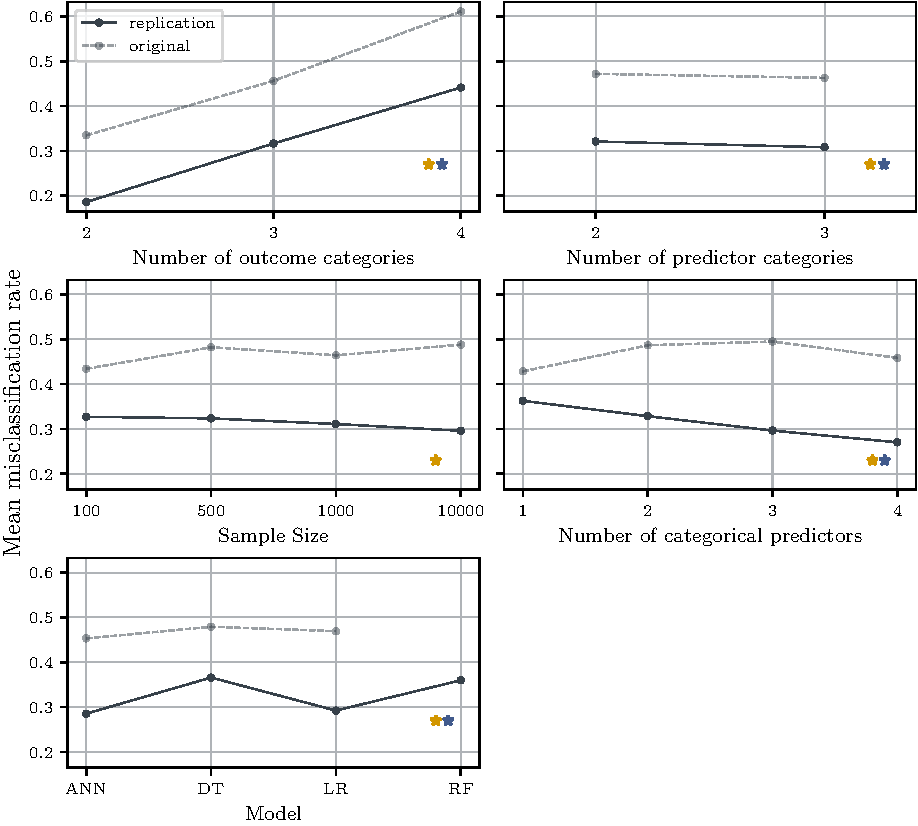
\includegraphics{fig/09_mainEffects_V5.pdf}
    \caption{Main Effects for Datasets with Five Predictors (Including Categorical Ones)}
    \label{fig:09_mainEffects_V5}
\end{figure}


\begin{figure}[h]
    \centering
    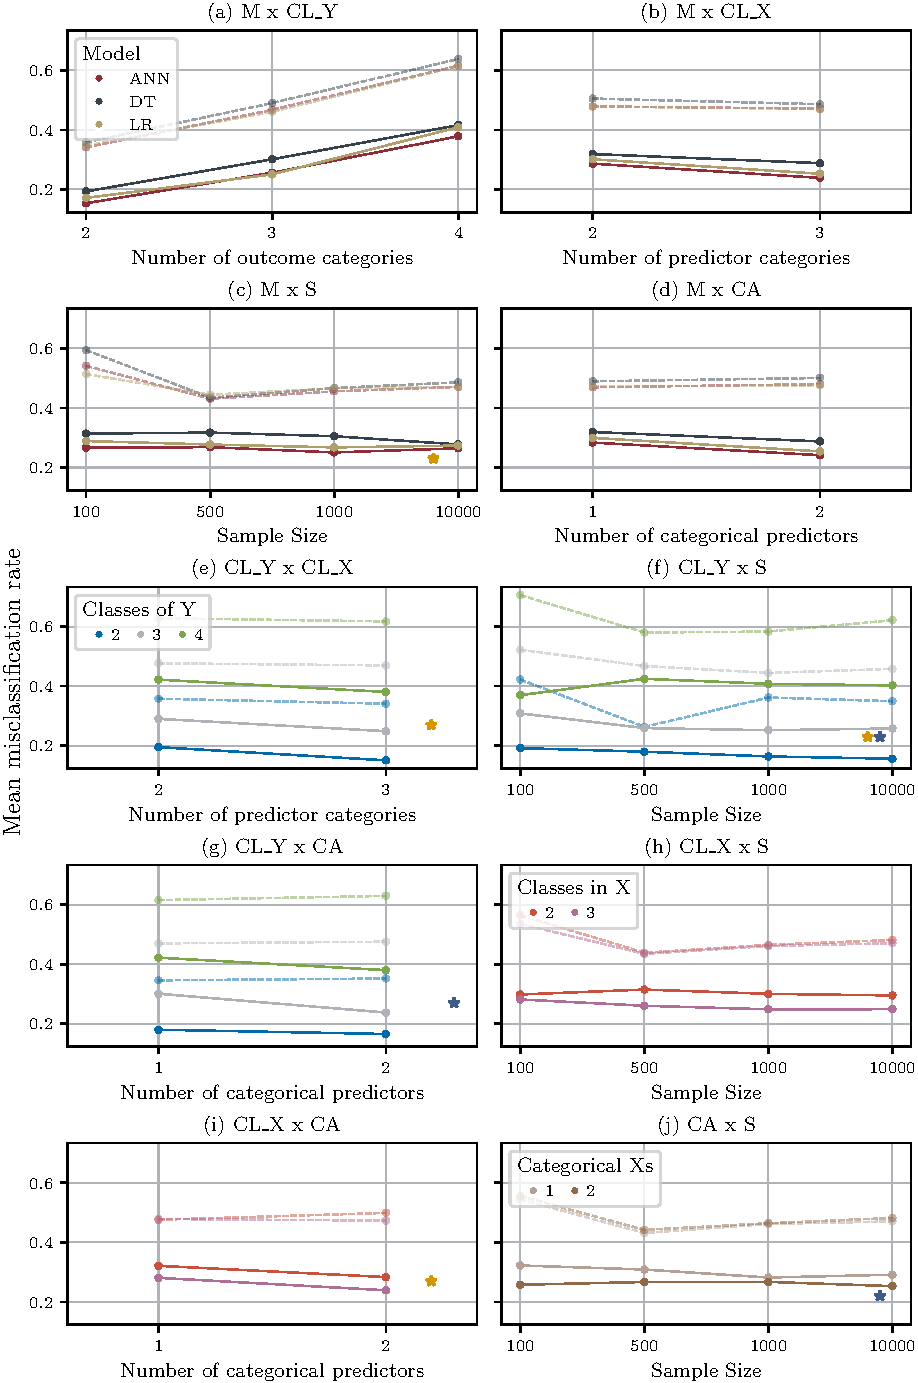
\includegraphics{fig/06_08_Interactions_V3.pdf}
    \caption{Interaction Plots for Datasets with Three Predictors}
    \label{fig:06_08_Interactions_V3}
\end{figure}

\begin{figure}[h]
    \centering
    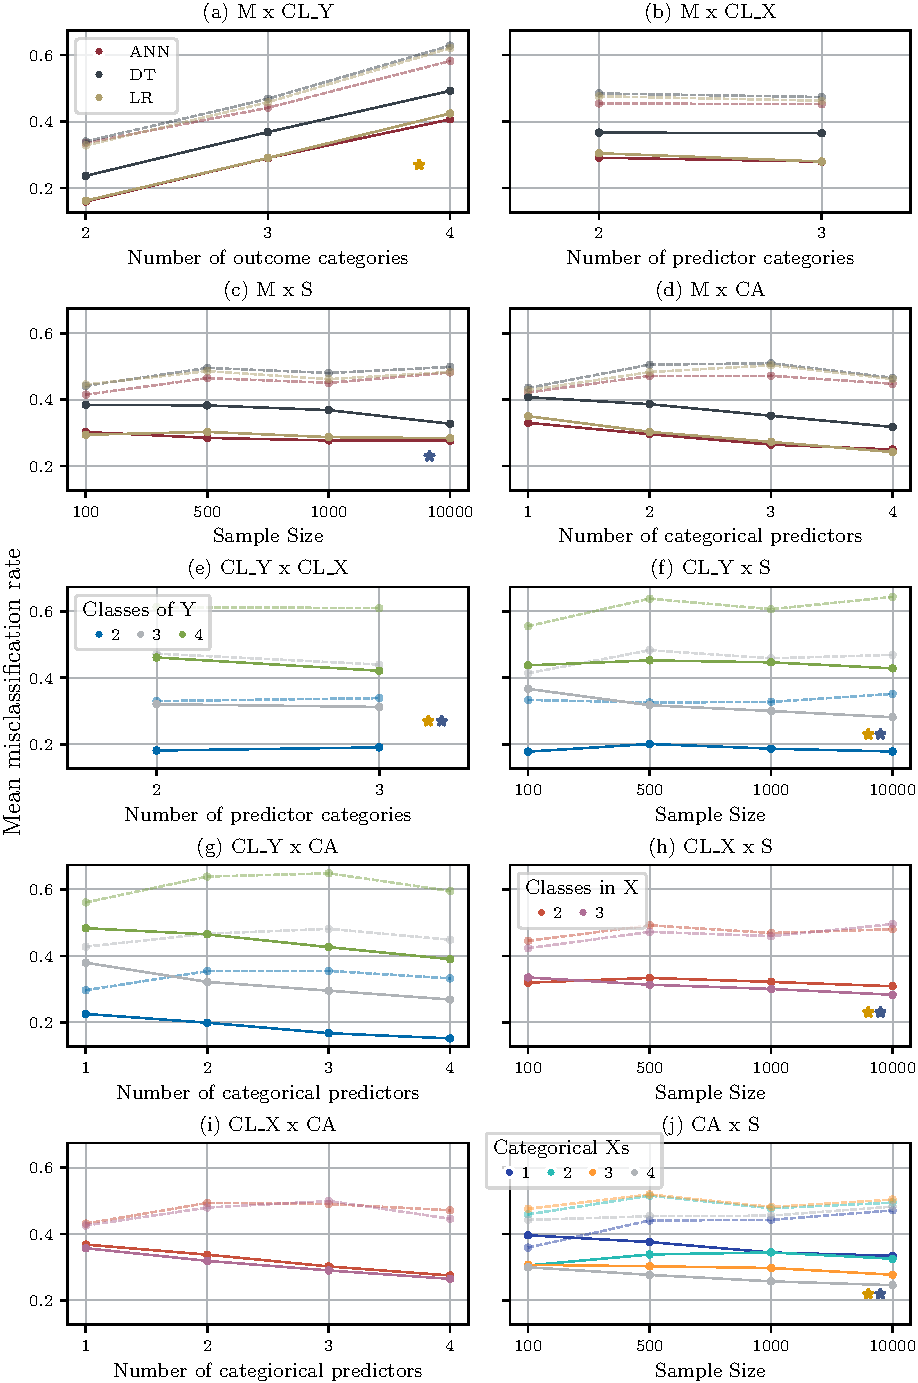
\includegraphics{fig/10_14_Interactions_V5.pdf}
    \caption{Interaction Plots for Datasets with Five Predictors}
    \label{fig:10_14_Interactions_V5}
\end{figure}

\begin{figure}[h]
    \centering
    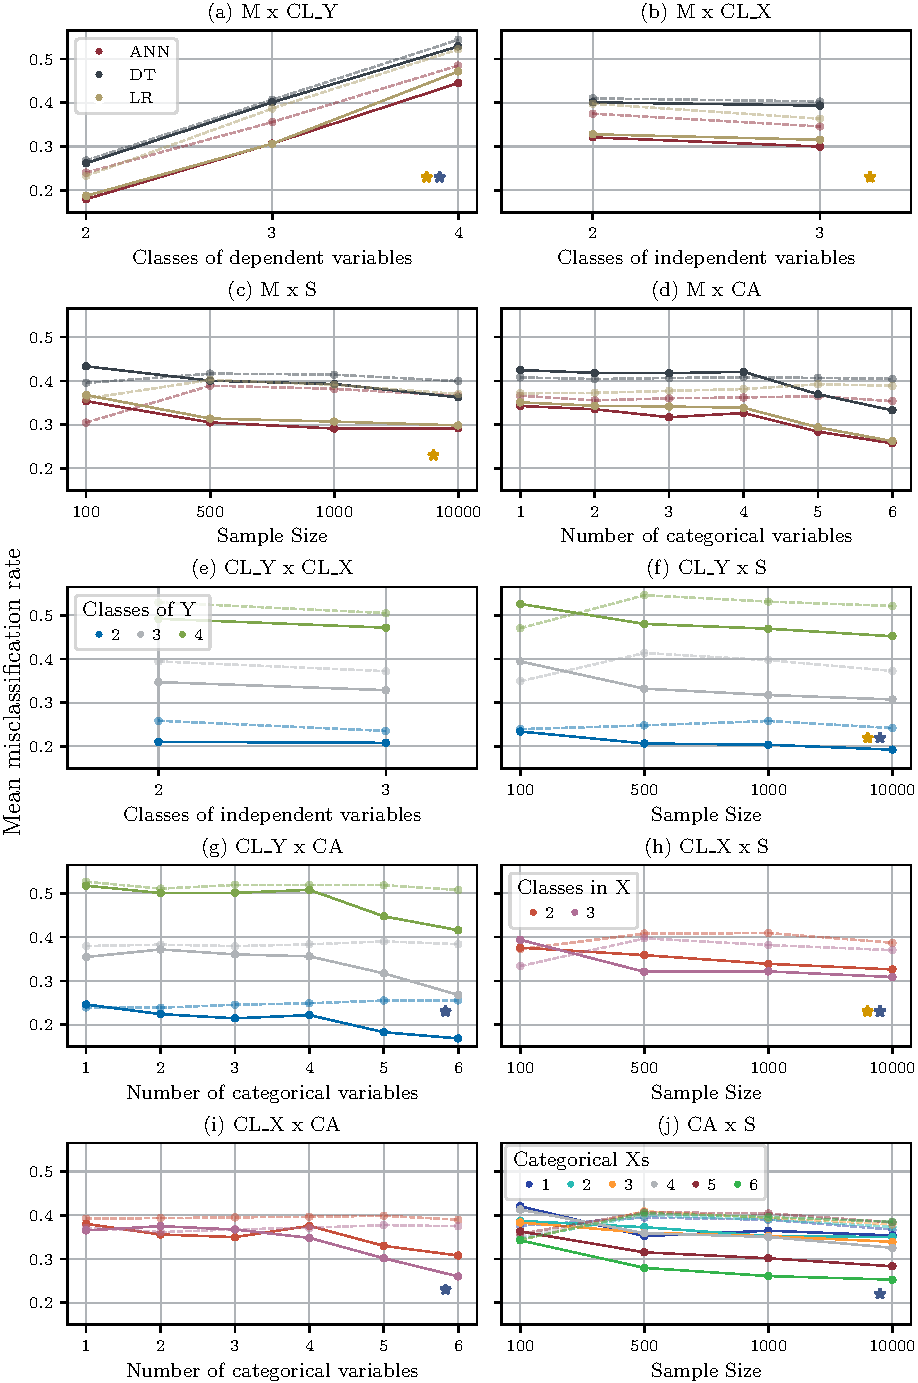
\includegraphics{fig/16_20_Interactions_V7.pdf}
    \caption{Interaction Plots for Datasets with Seven Predictors}
    \label{fig:16_20_Interactions_V7}
\end{figure}

% {\noindent \em Remainder omitted in this sample. See http://www.jmlr.org/papers/ for full paper.}

\end{document}
